\documentclass[10]{article}
\usepackage[titletoc, title]{appendix}
\usepackage{graphicx}
\usepackage{pdfpages}
%opening
\title{Software Design Document}
\author{Michael Farghali}

\begin{document}

\maketitle


\section{Introduction}
This Software Design Document (SSD) will give a very high overview of my Pascal complier which is based on the grammar rules given at the start of the course. The goal of this keystone course was to write a compiler in Java that accepts a text file representing a reduced version of Pascal. The text file will be scanned, parsed, converted into a syntax tree and finally written to an output file in assembly language. Upon completion of the course an executable .jar file should be submitted that does the above along with a user manual. 
 
\section{Scanner}

The purpose of the scanner class is to read in the source code and match all valid keywords and ids with their respective TokenType which are in the LookupTable class. It is based on a Deterministic Finite Automaton, Fig. \ref{fig: fg1}, and the given grammars seen in appendix \ref{grammars}. Each state in the DFA represents a state in the scanner. 
\begin{figure}[!ht]
	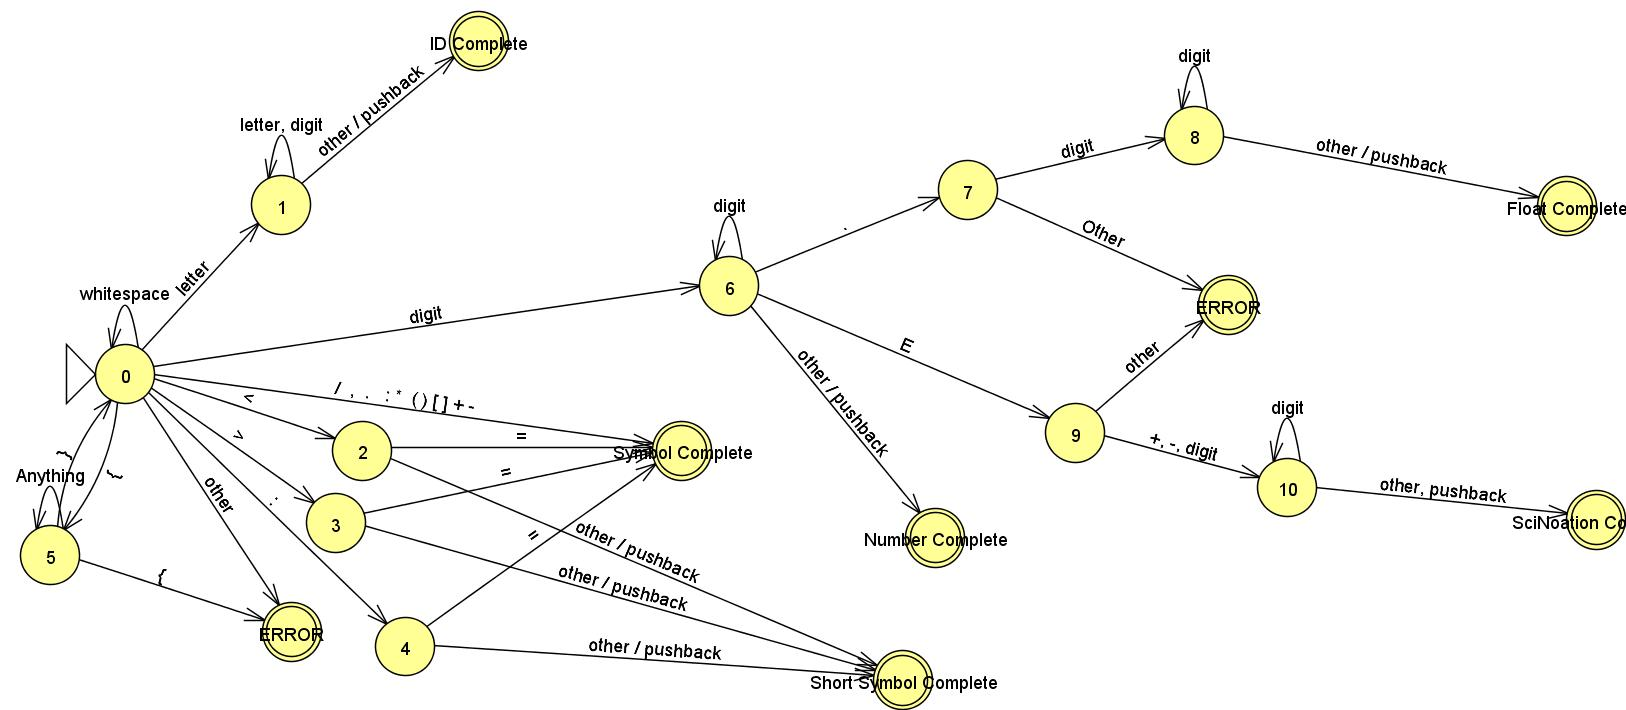
\includegraphics[width=\textwidth]{ScannerDFA.jpg}
	\caption{DFA \label{fig: fg1}}
	
\end{figure}

The scanner passes information to the Parser class primarily through the methods nextToken, getToken, and getLexeme. Most of the work done in the scanner class is done in the nextToken method which is responsible for checking that keywords are valid in our language and that IDs are also in a format allowed and returns true is so or false if not. The getToken method will be used by the parser to grab the current token from the scanner. Finally the getLexeme method is used to pass the name of a variable or invalid statement in the source code, to the parser. I chose to deviate from the example given in class and added methods \verb|pushBackChar()| and \verb|getNextChar()|. These methods don't do anything new but the code is used multiple times in the scanner class so I decided to create their own functions to clean up the nextToken method. I also added a method \verb|getCount()| which simply returns the line number where the scanner encounters an unexpected or invalid string. The UML for the scanner class can be seen below.

\begin{figure}[!ht]
	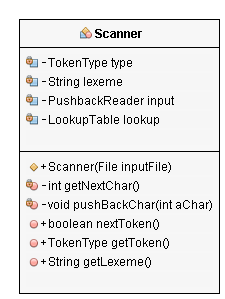
\includegraphics[height=3in]{ScannerUML.png}
	\caption{Scanner \label{fig: fg2}}
\end{figure}



\section{Parser}

The Parser class is responsible for a large portion of the work being done in this compiler. It uses the Context-Free grammar rules listed in Appendix \ref{grammars} and a push down automata to either accept or reject a source file. It uses top down recursive decent parsing which is convenient for implementation as all 24 nonterminal rules in our grammar become methods in the code. The UML diagram can be seen in appendix \ref{parserUML}. 

\paragraph{}
In the parser I also chose to deviate from the grammar given. I added methods \verb|addop()| and \verb|mulop()| which determine which kind of arithmetic or multiplication operator is being used. Adding these two functions helped to clean up the code and make in more readable in my opinion. I also deleted two methods, \verb|simple_part()| and \verb|term_part()| and added their functionality to \verb|simple_expression()| and \verb|term|. To me this seems more straightforward and easy to follow


\textbf{Add uml? ... }

\section{Symbol Table}

\section{Syntax Tree}

\textbf{Choosing to eliminate simple part....}

\section{Semantic Analysis}

\textbf{Bottom up recursive decent parsing for variable types?}
\textbf{Not using separate module}


\section{Code Generator}

\section{Conclusion}


\newpage
\begin{appendices}



\section{List of Keywords}
\label{keywords}
Symbols: $ . , - + * / ( ) { } [ ] { } < <= > >= : := ;$  
\newline
Keywords: div, mod, and, program, id, var, array, of, num, integer, real, function, procedure, begin, end, if, then, else, while, do, not

\section{Grammar Rules}
\label{grammars}
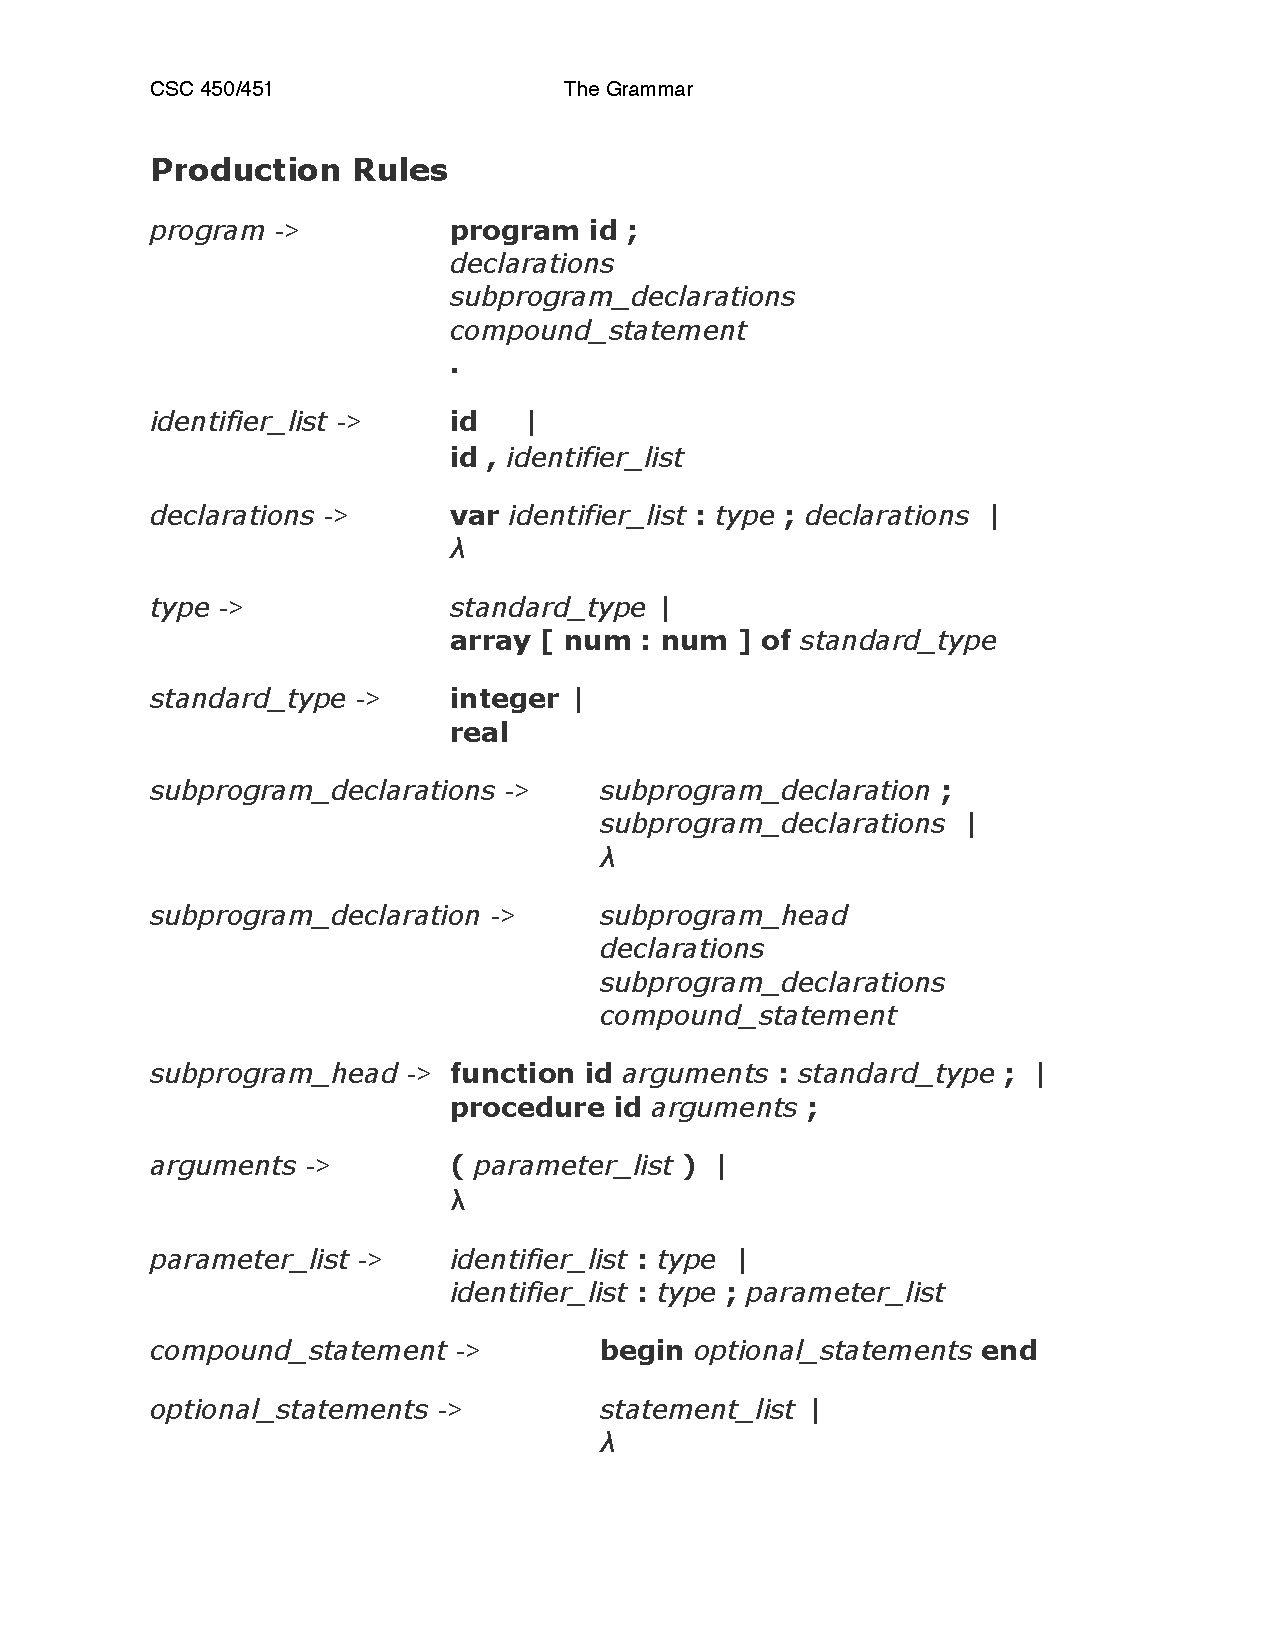
\includepdf[pages=-, scale=.8, noautoscale = true]{Grammar.pdf}


\begin{figure}
	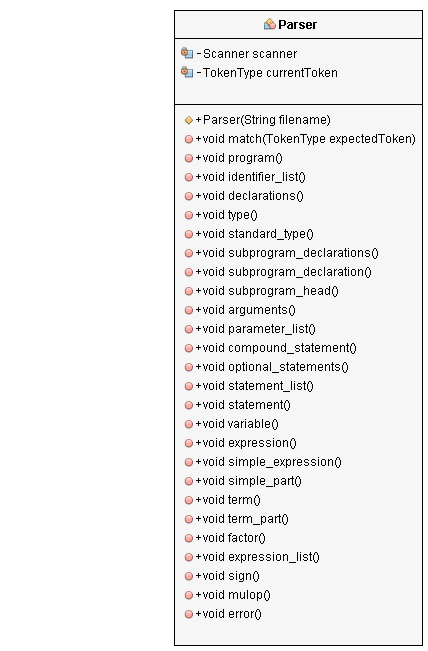
\includegraphics{ParserUML.png}
	\label{parserUML}
\end{figure}

\begin{figure}
	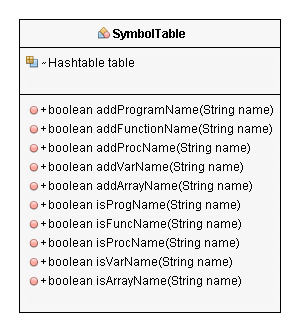
\includegraphics{SymTableUML.png}
\end{figure}

\end{appendices}


\end{document}
